\documentclass{article}

% Language setting
% Replace `english' with e.g. `spanish' to change the document language
\usepackage[polish]{babel}

% Set page size and margins
% Replace `letterpaper' with `a4paper' for UK/EU standard size
\usepackage[a4paper,top=2cm,bottom=2cm,left=3cm,right=3cm,marginparwidth=1.75cm]{geometry}

% Useful packages
\usepackage{amsmath}
\usepackage{graphicx}
\usepackage{listings}
\usepackage[pdftex,
            pdfauthor={Michał Czyż, Dawid Głąb},
            pdftitle={PK4 - Opis Projektu},
            pdfsubject={Opis Projektu},
            pdfkeywords={PK4, Projekt, Opis},
            pdfproducer={Latex with hyperref},
            pdfcreator={pdflatex},
            colorlinks=true,
            allcolors=blue]{hyperref}
\usepackage[T1]{fontenc}

\title{Projekt PK4: Platforma NLP}
\author{Michał Czyż}

\begin{document}
\maketitle

\section{Wstęp}

Projekt do wykonania w tym semestrze to platforma nlp. Jest to akronim od przetwarzania języka naturalnego \textit{(eng. natural langugage processing)}. W ramach projektu zaimplementowane zostanie tłumaczenie tekstu z jednego języka na drugi oraz badanie sentymentu, czyli ocena tekstu pod względem użytego słownictwa

\section{Opis projektu}

Projekt będzie się składał z trzech głównych części:

\begin{itemize}
  \item Core - napisany w C++, główna część programu analizująca sentyment i tłumacząca tekst.
  \item Middleware - serwer API, łączący komunikację między programem, a interfejsem sieciowym.
  \item Frontend - strona internetowa korzystająca z API aby komunikować się z programem, główna część odpowiedzialna za komunikację użytkownika z programem.
\end{itemize}

Założenie projektu jest bycie modularnym i dość prostym w rozbudowie. W szczególności, iż projekt jest dość złożony, i wymaga korzystania z wielu języków i bibliotek.

\section{Podział zadań}

Planowany jest następujący ogólny podział zadań. Jeśli chodzi o rdzeń programu, Dawid Głąb zajmie się badaniem sentymentu podawanego tekstu, natomiast Michał Czyż zajmie się tłumaczeniem podanego tekstu na wybrane języki. Każda z implementacji będzie spełniać wyamagania projektu, jakie były przewidziane na początku semestru. Jeśli chodzi o wartwę graficzną oraz komunikację pośrednią między interfejsem użytkownika, a samym programem w C++, Michał Czyż skupi się na bardziej na interfejsie od strony użytkownika, natomiast Dawid Głąb bardziej skupi swą uwagę nad stworzeniem poprawnego interfejsu API, między frontendem, a middlewarem. Planowane jest wykorzystanie różnych bibliotek w trakcie łączenia programu w C++ z Pythonem. 

\section{Opis problemu - tłumaczenie tekstu}

Problem tłumaczenia tekstu na wiele języków był trudny do zrealizowania przez długi czas. Model językowy musi potrafić nie tylko tłumaczyć odpowiadające wyrazy z jednego języka na drugi, ale także znać zasady gramatyczne panujące w danum języku oraz kontekst, gdyż to samo zdanie w wielu przypadkach może mieć różne znaczenia. 

Moim sposobem na rozwiązanie tego problemu jest wykorzystanie gotowych, wytrenowanych modelów dostępnych online i następnie spróbować oprogramować je w C++, aby możliwa była interakcja i tłumaczenie tekstu z jednego języka na drugi. Chciałbym także dodać możliwośc detekcji języka, aby podany tekst był wykrywany automatycznie, przez co pozwoli na wygodniejsze użycie. 

Sam problem tłumacznia wymaga wytrenowania datasetu nlp. Spróbuję wykorzystać zbiór \textit{kde4}, gdyż wspiera wiele języków. Istanieje także dostosowanie i dotrenowanie tego zbioru danych aby osiągnąć lepsze wyniki dla konktretnej pary. Oprócz tego, spróbuję wykorzystać CTranslate2, aby móc wykorzystywać tłumaczenie za pomocą \textit{llm} jak to robi na przykład projekt OpenAI Whisper.

Głównym problemem jest znaleźć dobrą bibliotekę która prawidłowo obsłuży komunikację z modelem w c++, oraz zbudowanie odpowiedniej abstrakcji klas, która pozwoli na wygodną komunikację i modułowość. 

Dane wejściowe do programu to będzie podane przez gRPC lub podobny protokół, tekst, który chcemy aby został przetłumaczony, oraz język źródłowy i docelowy. W przypadku wykrywania języka będzie jakiś sposób zapisu, który odróżni go od innych. 

\section{Wykorzystane technologie}

Projekt będzie wykorzystywał trzy języki programowania. 

\begin{itemize}
  \item Głowna część projektu będzie stworzona w C++ z wykorzystaniem gRPC do komunikacji. Część C++ będzie stworzona obiektowo i zawierać będzie większość wymagań projektu. 
  \item Część pośrednia (middleware backend), będzie napisana w Pythonie, z wykorzystaniem Flaska, jako frameworka serwerowego. 
  \item Część użytkownika (frontend) będzie napisana w JavaScripcie, a w szczególności wykorzystwać będzie framework React wraz z Next.JS. Warstwa wizualna będzie wykorzystywała framework CSS \textit{halfmoon}. 
\end{itemize}

\section{Wykorzystane zagadnienia z laboratorium}

Zagadnienia wykorzystane z laboratorium w ramach projektu, które w tej chwili uważam, że zostaną wykorzystane to: asynchroniczność, gdyż potrzebna będzie implementacja asynchronicznej komunikacji między modelem, a samym interfejsem aplikacji obsługującym requesty; wątkowość, ponieważ może się okazać konieczne korzystanie z wielu instancji programu w celu ułatwienia wydajności i umożliwienie tłumaczenie z wielu klientów webowych jednocześnie. Chcę także wykorzystać wyrażenia regularne, aby znajdować ewentualne dane osobowe i je anonimizować, to znaczy losować z jakiś ogólnych danych aby uniknąć utraty danych osobowych. Zagadnieniem z laboratorium także wykorzystywanym będzie dostęp do systemu plików, gdyż będzie potrzebna umiejętność ładowania modelu do programu, oraz ewentualne operacje zapisuwania logów z przebiegu działania programu.

\section{Propozycja interfejsu użytkownika}

Przygotowany został początkowy mockup UI. 
Interfejs składa się z nagłówka i panelu bocznego z poziomu którego będą dostępne tryby aplikacji wraz z ich ustawieniami. W głównym oknie będą pojawiać się konkretne elementy UI do interakcji z programem.

\begin{figure}
\centering
  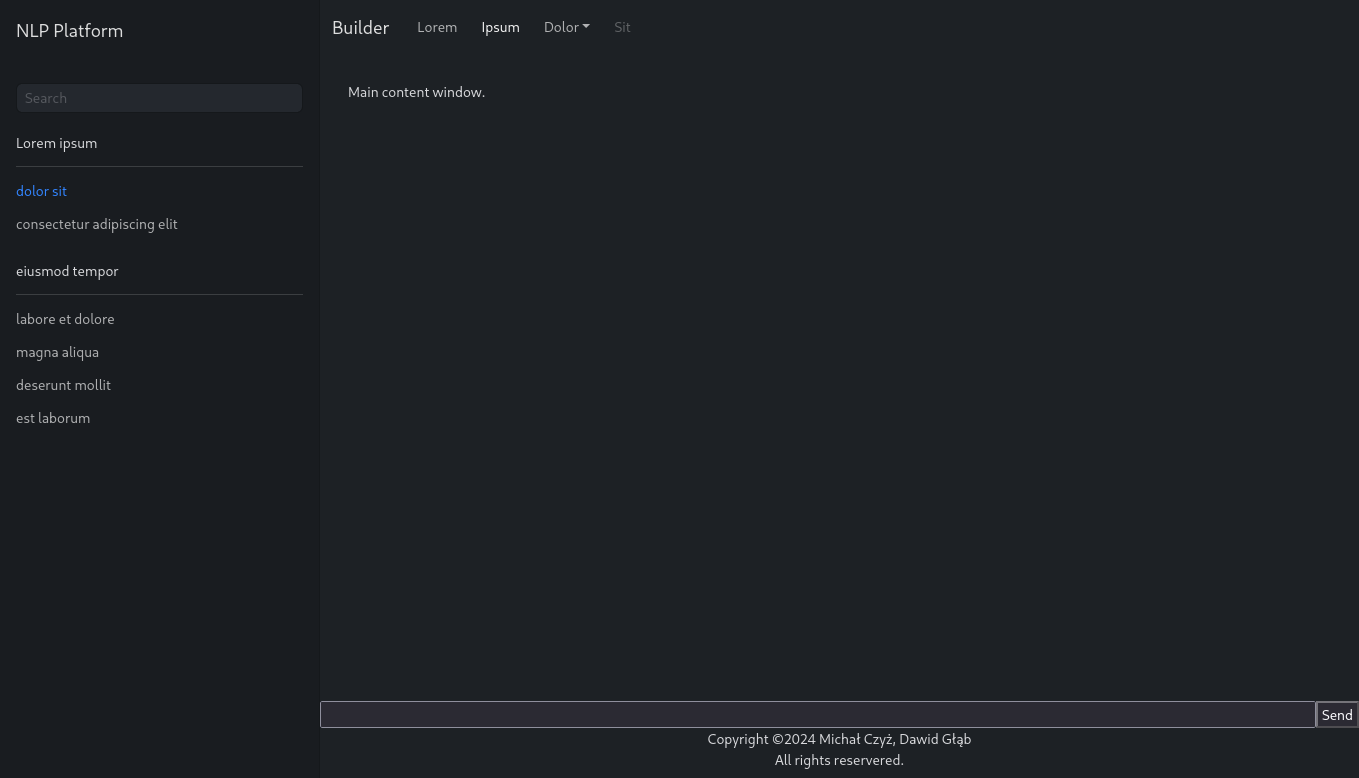
\includegraphics[width=1\linewidth]{ui_mockup.png}
  \caption{\label{fig:ui mockup}Propozycja interfejsu użytkownika.}
\end{figure}

Sam program w C++ nie będzie posiadał wartwy graficznej, a tylko interfejs tekstowy pozwalający na podgląd czy połączenia z Pythonem przebiegają prawidłową. Czyli serwer słuchający na porcie i logujący requesty. Podobnie będzie z wartwą pośrednią napisaną w Pythonie. Będzie ona nasłuchiwać na zapytania z internetu i przekazywać je do głównego programu w C++. Ale dla strony Pythona, z tego powodu, że jest on pośrednikiem z częścią webową, także będzie wspierał surowe requesty po API, co pozwala na wykorzystanie platformy nie tylko poprzez interfejs graficzny, ale także pozwala na uniwersalne wykorzystanie programu, dalej przez innnych programistów. Co z założenia ułatwia dostęp do aplikacji i wzbogaca modularność. 

Interfejs graficzny będzie głównie po stronie webowej. Jak zaprezentowano na rysunku.

Natomiast interfejs API będzie się komunikować jako request. Poniżej propzycja dla tłumaczenia tekstu w formie JSONa:

\begin{lstlisting}
{
  type: "<operation_type>",
  input: "<input_text>",
  output: "<output_text>",
  mods: {
    src: "<source_langugage>", 
    dst: "<destination_language>",
    anon: "<anonymize_data>"
  }
}
\end{lstlisting}

\end{document}
